\documentclass[]{article}
\usepackage{lmodern}
\usepackage{amssymb,amsmath}
\usepackage{ifxetex,ifluatex}
\usepackage{fixltx2e} % provides \textsubscript
\ifnum 0\ifxetex 1\fi\ifluatex 1\fi=0 % if pdftex
  \usepackage[T1]{fontenc}
  \usepackage[utf8]{inputenc}
\else % if luatex or xelatex
  \ifxetex
    \usepackage{mathspec}
  \else
    \usepackage{fontspec}
  \fi
  \defaultfontfeatures{Ligatures=TeX,Scale=MatchLowercase}
\fi
% use upquote if available, for straight quotes in verbatim environments
\IfFileExists{upquote.sty}{\usepackage{upquote}}{}
% use microtype if available
\IfFileExists{microtype.sty}{%
\usepackage{microtype}
\UseMicrotypeSet[protrusion]{basicmath} % disable protrusion for tt fonts
}{}
\usepackage[margin=1in]{geometry}
\usepackage{hyperref}
\hypersetup{unicode=true,
            pdftitle={Dados CEPEA},
            pdfauthor={Lucca Simeoni Pavan  João Carlos de Carvalho},
            pdfborder={0 0 0},
            breaklinks=true}
\urlstyle{same}  % don't use monospace font for urls
\usepackage{graphicx,grffile}
\makeatletter
\def\maxwidth{\ifdim\Gin@nat@width>\linewidth\linewidth\else\Gin@nat@width\fi}
\def\maxheight{\ifdim\Gin@nat@height>\textheight\textheight\else\Gin@nat@height\fi}
\makeatother
% Scale images if necessary, so that they will not overflow the page
% margins by default, and it is still possible to overwrite the defaults
% using explicit options in \includegraphics[width, height, ...]{}
\setkeys{Gin}{width=\maxwidth,height=\maxheight,keepaspectratio}
\IfFileExists{parskip.sty}{%
\usepackage{parskip}
}{% else
\setlength{\parindent}{0pt}
\setlength{\parskip}{6pt plus 2pt minus 1pt}
}
\setlength{\emergencystretch}{3em}  % prevent overfull lines
\providecommand{\tightlist}{%
  \setlength{\itemsep}{0pt}\setlength{\parskip}{0pt}}
\setcounter{secnumdepth}{5}
% Redefines (sub)paragraphs to behave more like sections
\ifx\paragraph\undefined\else
\let\oldparagraph\paragraph
\renewcommand{\paragraph}[1]{\oldparagraph{#1}\mbox{}}
\fi
\ifx\subparagraph\undefined\else
\let\oldsubparagraph\subparagraph
\renewcommand{\subparagraph}[1]{\oldsubparagraph{#1}\mbox{}}
\fi

%%% Use protect on footnotes to avoid problems with footnotes in titles
\let\rmarkdownfootnote\footnote%
\def\footnote{\protect\rmarkdownfootnote}

%%% Change title format to be more compact
\usepackage{titling}

% Create subtitle command for use in maketitle
\newcommand{\subtitle}[1]{
  \posttitle{
    \begin{center}\large#1\end{center}
    }
}

\setlength{\droptitle}{-2em}
  \title{Dados CEPEA}
  \pretitle{\vspace{\droptitle}\centering\huge}
  \posttitle{\par}
  \author{Lucca Simeoni Pavan \hspace{1cm} João Carlos de Carvalho}
  \preauthor{\centering\large\emph}
  \postauthor{\par}
  \predate{\centering\large\emph}
  \postdate{\par}
  \date{\today}

\setlength\parindent{24pt}
\usepackage[english, brazil]{babel}
\usepackage[utf8]{inputenc}
\usepackage{longtable}
\usepackage{booktabs}

\begin{document}
\maketitle

Os dados são de peridiocidade diária e são disponibilizados pela
\href{http://www.cepea.esalq.usp.br/br/consultas-ao-banco-de-dados-do-site.aspx}{CEPEA/EXALQ}
e se referem ao período de a 23/01/2017. O dados para o etanol
correspondem ao Indicador Diário do Etanol Hidratado ESALQ/BM\&FBovespa
Posto Paulínia (SP). Para o açúcar os dados são o Indicado Açúcar
Criatal CEPEA/EXALQ - São Paulo por saca de 50 quilos. Para o soja os
dados são o Indicador Soja CEPEA/EXALQ - Paraná por saca de 60 quilos.
Ocorreram 15 valores faltante para o soja durante o período que foram
interpolados pelo método \emph{spline} conforme indicado por Zeileis and
Grothendieck (2005).

\begin{longtable}[t]{lllll}
\caption{\label{tab:unnamed-chunk-5}Resumo das séries de preços}\\
\toprule
  &     acucar &     etanol &      soja &      Data\\
\midrule
 & Min.   :32.97 & Min.   : 732.5 & Min.   : 39.99 & Min.   :2010-01-25\\
 & 1st Qu.:48.25 & 1st Qu.:1105.1 & 1st Qu.: 49.13 & 1st Qu.:2011-10-20\\
 & Median :63.17 & Median :1190.5 & Median : 53.92 & Median :2013-07-24\\
 & Mean   :61.47 & Mean   :1238.0 & Mean   : 59.97 & Mean   :2013-07-23\\
 & 3rd Qu.:73.06 & 3rd Qu.:1317.0 & 3rd Qu.: 71.58 & 3rd Qu.:2015-04-23\\
 & Max.   :93.18 & Max.   :1924.5 & Max.   :100.92 & Max.   :2017-01-20\\
\bottomrule
\end{longtable}

Para vizualização dos dados foi plotado na Figura 1 os gráficos do log
da série de preços e do log da série de preços deflacionada. Optou-se
pela apresentação na forma de logarítmo devido a diferença de escala
entre o preço do etanol e dos preços da soja e açúcar. Na Figura 2
consta a volatilidade \(v_i\) do etanol, açúcar e soja medida pela
seguinte fórmula:

\[v_i = \bigg(\Delta \log p_{i,t}\bigg)^2.\] Em que \(p_{i,t}\) é o
preço da \emph{commodity} \(i\) e \(i = \text{etanol, açúcar ou soja}\).
Percebe-se que a volatilidade do preço do açúcar é bem mais intensa e
com maior amplitude se comparadas às volatilidades do preço do soja e do
preço do etanol. Entretanto, conforme López Cabrera and Schulz (2016) é
característico das séries de preços de \emph{commodities} serem
cointegradas e uma medida de volatilidade que leve em conta esta
característica dos dados se torna mais apropriada. Para isso pode-se
modelar a média da série de preços por meio e um modelo de correção de
erros (VECM, sigla em inglês) e então filtrar a série de preços do
co-movimento de suas médias condicionais.

\begin{figure}[htbp]
\centering
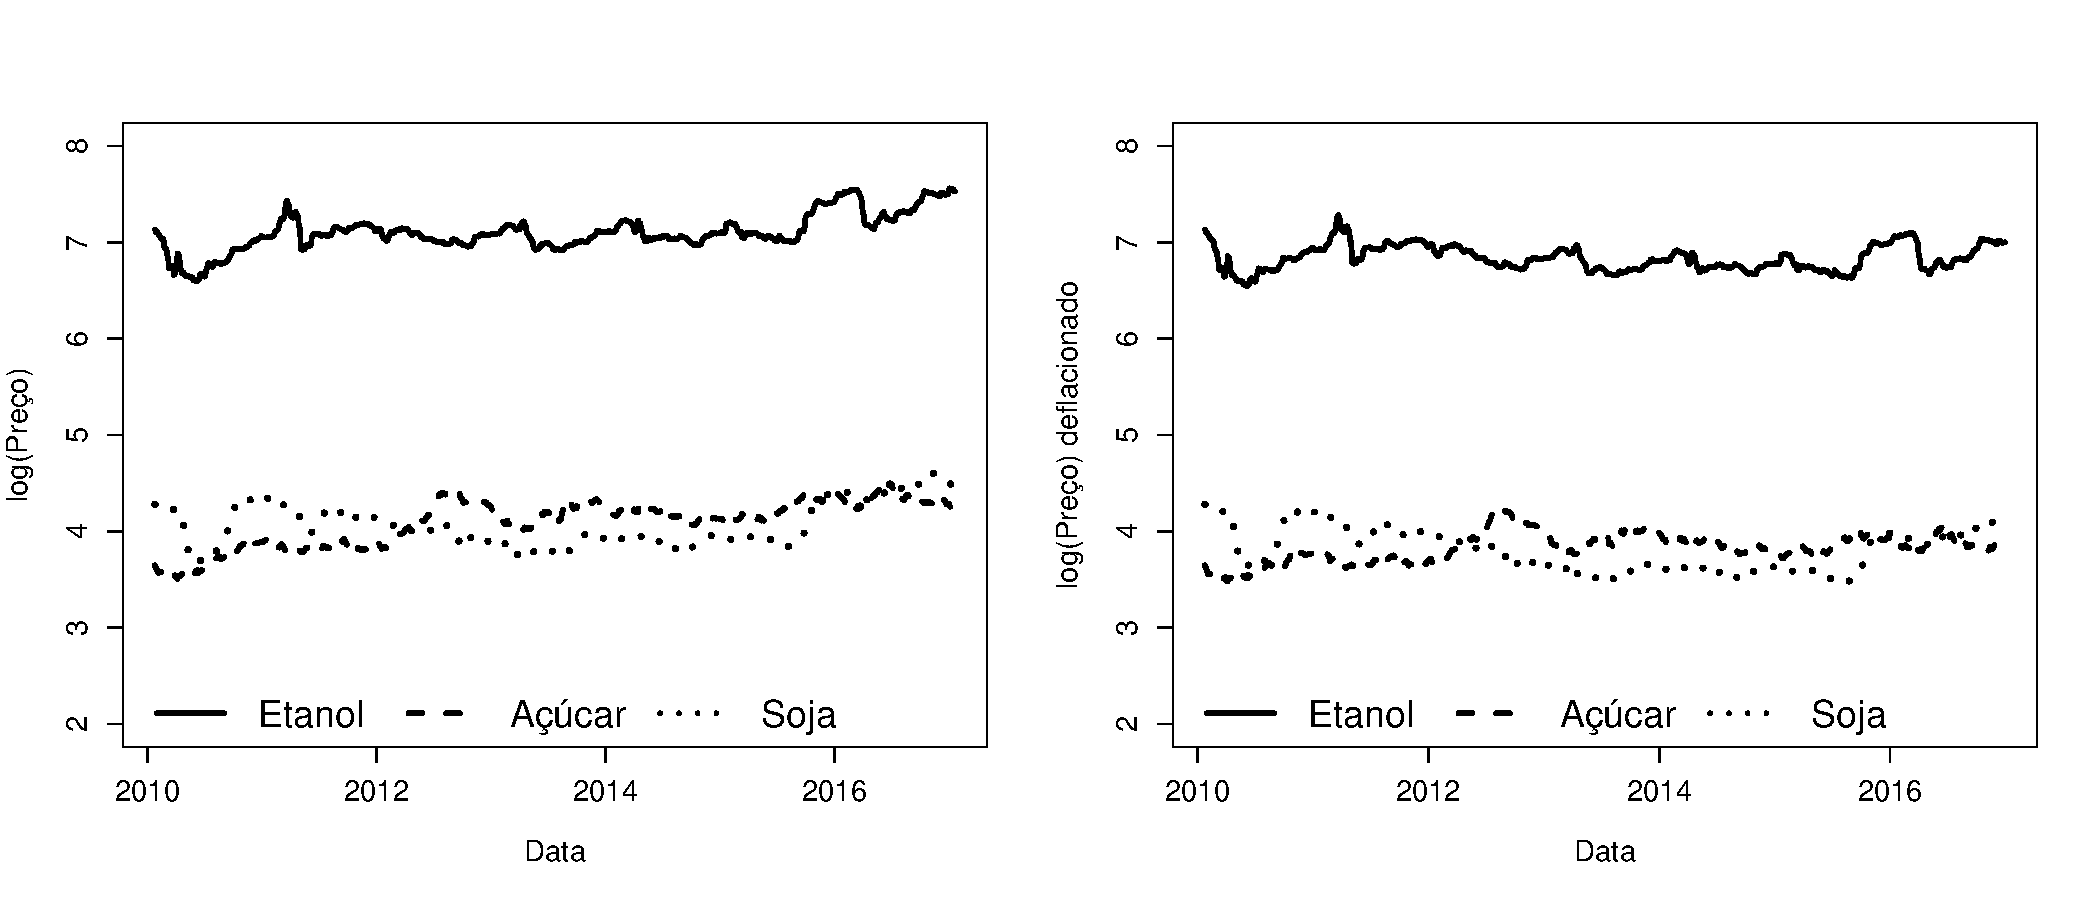
\includegraphics{dados_cepea_files/figure-latex/grafico1-1.pdf}
\caption{Logarítimo dos preços diários e preço diário deflacionado pelo
Ìndice de Preço do Produtor (IPP) para o etanol, açúcar e soja}
\end{figure}

\begin{figure}[htbp]
\centering
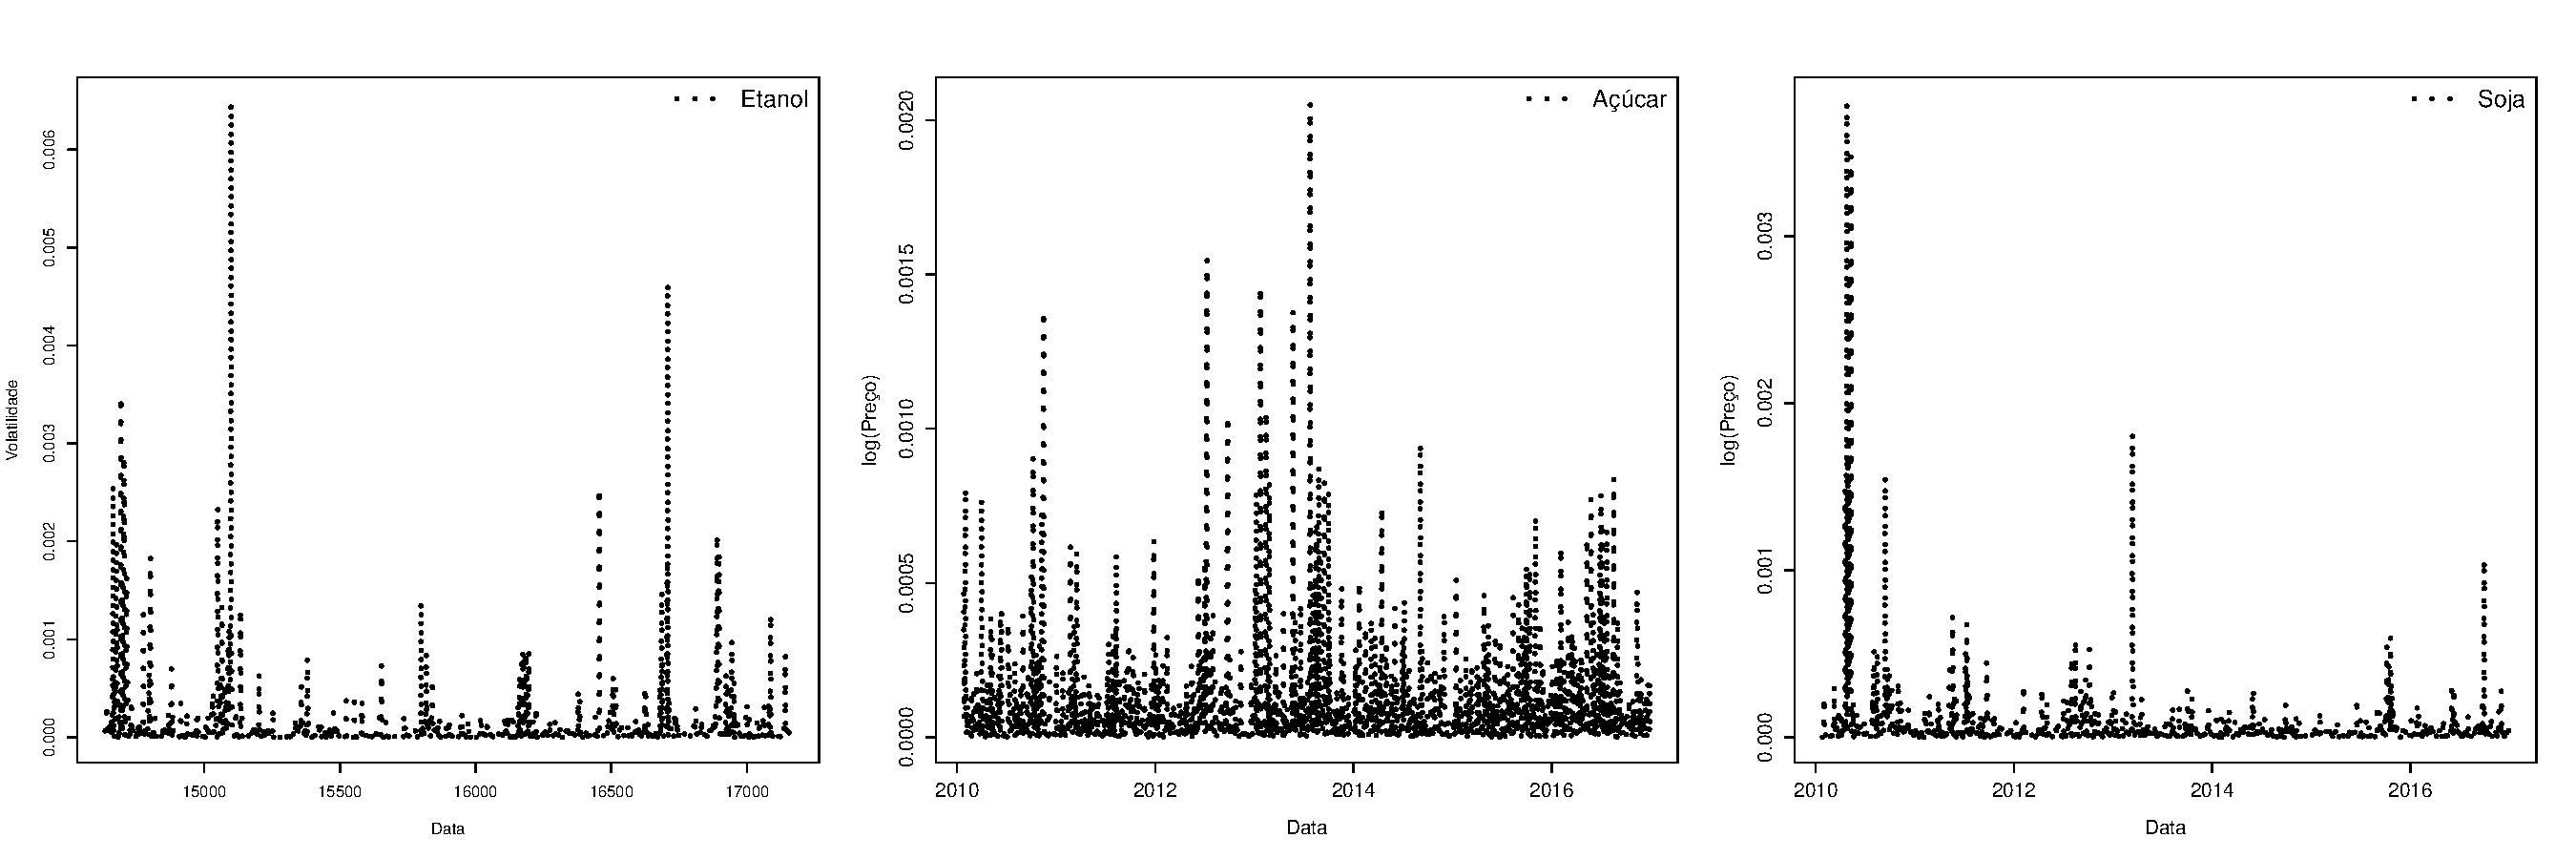
\includegraphics{dados_cepea_files/figure-latex/grafico2-1.pdf}
\caption{Volatilidade medida pela diferença do logarítimo do preço ao
quadrado para a etanol, açúcar e soja}
\end{figure}

\begin{verbatim}
## [1] "Mean"
\end{verbatim}

\begin{verbatim}
##   etanol   acucar     soja 
## 6.835560 3.825533 3.799046
\end{verbatim}

\begin{verbatim}
## [1] "St.D."
\end{verbatim}

\begin{verbatim}
##           etanol    acucar      soja
## etanol 0.1308831       NaN 0.1344304
## acucar       NaN 0.1462893       NaN
## soja   0.1344304       NaN 0.2241026
\end{verbatim}

\begin{verbatim}
## [1] "Corr."
\end{verbatim}

\begin{verbatim}
##           etanol     acucar       soja
## etanol  1.000000 -0.1788200  0.6161190
## acucar -0.178820  1.0000000 -0.4055711
## soja    0.616119 -0.4055711  1.0000000
\end{verbatim}

\begin{verbatim}
## [1] "Skewness"
\end{verbatim}

\begin{verbatim}
## [1] -0.2896277 -0.1595681 -1.0635649
\end{verbatim}

\begin{verbatim}
## [1] "Kurtosis"
\end{verbatim}

\begin{verbatim}
## [1] 12.333846  4.283914 12.858063
\end{verbatim}

\begin{verbatim}
## [1] "Box Ljung (residuals)"
\end{verbatim}

\begin{verbatim}
## [1] 0.000000e+00 5.107026e-15 0.000000e+00
\end{verbatim}

\begin{verbatim}
## [1] "Box-Ljung (squared residuals)"
\end{verbatim}

\begin{verbatim}
## [1] 0.000000e+00 2.233032e-07 0.000000e+00
\end{verbatim}

\begin{verbatim}
## [1] "ARCH"
\end{verbatim}

\begin{verbatim}
##  Chi-squared  Chi-squared  Chi-squared 
## 0.0000000000 0.0006158753 0.0000000000
\end{verbatim}

\begin{verbatim}
## [1] "Shapiro-Wilk"
\end{verbatim}

\begin{verbatim}
## [1] 3.767565e-36 7.597055e-10 2.443580e-30
\end{verbatim}

\begin{longtable}[t]{lrrrrrrr}
\caption{\label{tab:ADF e KPSS nivel}Teste KPSS preço em nível}\\
\toprule
  & etanol & acucar & soja & 1 Pct & 2.5 Pct & 5 Pct & 10 Pct\\
\midrule
Time Trend: & 1.57 & 3.80 & 5.17 & 0.22 & 0.18 & 0.15 & 0.12\\
No Trend: & 1.88 & 10.65 & 9.45 & 0.74 & 0.57 & 0.46 & 0.35\\
\bottomrule
\end{longtable}

\begin{longtable}[t]{lrrrrrrr}
\caption{\label{tab:ADF e KPSS nivel}Teste ADF preço em nível}\\
\toprule
  & etanol & acucar & soja & 1 Pct & 2.5 Pct & 5 Pct & 10 Pct\\
\midrule
Time Trend: & -3.83 & -1.67 & -2.44 & -3.96 & -3.66 & -3.41 & -3.12\\
Constant: & -3.87 & -1.90 & -2.67 & -3.43 & -3.12 & -2.86 & -2.57\\
Neither: & -0.16 & 0.27 & -0.39 & -2.58 & -2.23 & -1.95 & -1.62\\
\bottomrule
\end{longtable}

\begin{longtable}[t]{lrrr}
\caption{\label{tab:ADF e KPSS nivel}Defasagens do teste ADF}\\
\toprule
  & Trend Model & Drift Model & None\\
\midrule
etanol & 2 & 2 & 2\\
acucar & 1 & 1 & 1\\
soja & 6 & 6 & 5\\
\bottomrule
\end{longtable}

\begin{verbatim}
## 
##  Phillips-Perron Unit Root Test
## 
## data:  dados_cepea_deflacionado[, "etanol"]
## Dickey-Fuller Z(alpha) = -18.985, Truncation lag parameter = 8,
## p-value = 0.08703
## alternative hypothesis: stationary
\end{verbatim}

\begin{verbatim}
## 
##  Phillips-Perron Unit Root Test
## 
## data:  dados_cepea_deflacionado[, "acucar"]
## Dickey-Fuller Z(alpha) = -6.7393, Truncation lag parameter = 8,
## p-value = 0.7338
## alternative hypothesis: stationary
\end{verbatim}

\begin{verbatim}
## 
##  Phillips-Perron Unit Root Test
## 
## data:  dados_cepea_deflacionado[, "soja"]
## Dickey-Fuller Z(alpha) = -3.9061, Truncation lag parameter = 8,
## p-value = 0.8919
## alternative hypothesis: stationary
\end{verbatim}

\begin{longtable}[t]{lrrrrrrr}
\caption{\label{tab:ADF e KPSS logdif}Teste KPSS retorno}\\
\toprule
  & etanol & acucar & soja & 1 Pct & 2.5 Pct & 5 Pct & 10 Pct\\
\midrule
Time Trend: & 0.05 & 0.06 & 0.11 & 0.22 & 0.18 & 0.15 & 0.12\\
No Trend: & 0.15 & 0.14 & 0.72 & 0.74 & 0.57 & 0.46 & 0.35\\
\bottomrule
\end{longtable}

\begin{longtable}[t]{lrrrrrrr}
\caption{\label{tab:ADF e KPSS logdif}Teste ADF retorno}\\
\toprule
  & etanol & acucar & soja & 1 Pct & 2.5 Pct & 5 Pct & 10 Pct\\
\midrule
Time Trend: & -15.51 & -25.43 & -9.18 & -3.96 & -3.66 & -3.41 & -3.12\\
Constant: & -15.49 & -25.42 & -9.11 & -3.43 & -3.12 & -2.86 & -2.57\\
Neither: & -15.50 & -25.42 & -9.11 & -2.58 & -2.23 & -1.95 & -1.62\\
\bottomrule
\end{longtable}

\begin{longtable}[t]{lrrr}
\caption{\label{tab:ADF e KPSS logdif}Defasagens do teste ADF}\\
\toprule
  & Trend Model & Drift Model & None\\
\midrule
etanol & 1 & 1 & 1\\
acucar & 1 & 1 & 1\\
soja & 4 & 4 & 4\\
\bottomrule
\end{longtable}

\begin{verbatim}
## 
##  Phillips-Perron Unit Root Test
## 
## data:  ldif_cepea[-1, "etanol"]
## Dickey-Fuller Z(alpha) = -990.04, Truncation lag parameter = 8,
## p-value = 0.01
## alternative hypothesis: stationary
\end{verbatim}

\begin{verbatim}
## 
##  Phillips-Perron Unit Root Test
## 
## data:  ldif_cepea[-1, "acucar"]
## Dickey-Fuller Z(alpha) = -1473.5, Truncation lag parameter = 8,
## p-value = 0.01
## alternative hypothesis: stationary
\end{verbatim}

\begin{verbatim}
## 
##  Phillips-Perron Unit Root Test
## 
## data:  ldif_cepea[-1, "soja"]
## Dickey-Fuller Z(alpha) = -1685.5, Truncation lag parameter = 8,
## p-value = 0.01
## alternative hypothesis: stationary
\end{verbatim}

\pagebreak

\section*{Referências}\label{referencias}
\addcontentsline{toc}{section}{Referências}

\setlength{\parindent}{0in}

\hypertarget{refs}{}
\hypertarget{ref-lopez_cabrera_volatility_2016}{}
López Cabrera, Brenda, and Franziska Schulz. 2016. ``Volatility Linkages
Between Energy and Agricultural Commodity Prices.'' \emph{Energy
Economics} 54 (February): 190--203.
doi:\href{https://doi.org/10.1016/j.eneco.2015.11.018}{10.1016/j.eneco.2015.11.018}.

\hypertarget{ref-zeileis_zoo:_2005}{}
Zeileis, Achim, and Gabor Grothendieck. 2005. ``Zoo: S3 Infrastructure
for Regular and Irregular Time Series.'' \emph{Journal of Statistical
Software} 014 (i06): 1--27.
doi:\href{https://doi.org/10.18637/jss.v014.i06}{10.18637/jss.v014.i06}.


\end{document}
